\subsection{Descripci\'on del problema}

En este ejercicio se nos pide escribir un algoritmo que resuelva una especie de rompecabezas dado por un tablero de $n \times m$ casillas y $n \times m$ fichas.
Cada pieza (cuadrada) tiene un color en cada uno de sus lados, no necesariamente colores distintos en cada uno. Por ejemplo: 

\begin{figure}[h]
\begin{center}
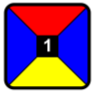
\includegraphics[scale=0.4]{./img/ej3_fichas.png}
\caption{Ejemplo de ficha}
\end{center}
\end{figure}

Ahora, para poder poner una pieza en el tablero debemos asegurarnos de que los colores de los lados coincidan con los de las fichas adyacentes (en caso de que haya una ficha lindante). Un ejemplo de las posicionamiento correcto e incorrecto ser\'ia:\\

\begin{figure}[h]
\begin{center}
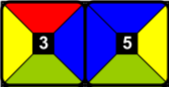
\includegraphics[scale=0.4]{./img/ej3_fichas_coinciden.png}
\caption{Ejemplo posicionamiento correcto}
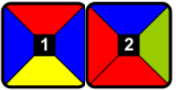
\includegraphics[scale=0.4]{./img/ej3_fichas_ncoinciden.png}
\caption{Ejemplo posicionamiento incorrecto}
\end{center}
\end{figure}

Adem\'as no se pueden girar las piezas por más que esto permita llegar a una mejor soluci\'on.\\
M\'as all\'a de estas restricciones, cualquier pieza puede colocarse en cualquier casillero.\\
La soluci\'on entregada por el algoritmo no necesariamente debe tener el tablero lleno, ya que con el conjunto de piezas dado podr\'ia no existir una forma de ubicarlas todas cumpliendo con lo pedido. Por lo tanto, la soluci\'on al problema debe ser lo m\'as \'optima posible: aquella en la que mayor cantidad de piezas permita ingresar en el tablero dadas las restricciones anteriores.
Por ejemplo el siguiente gr\'afico muestra una soluci\'on \'optima, dado un conjunto de piezas que no permiten llenar por completo el tablero.

/*Imagen editada del enunciado*/

\subsection{Resoluci\'on}

Para resolver este problema se nos pidi\'o utilizar la t\'ecnica algor\'itmica de backtracking.\\ 
Comenzamos situados en el primer casillero (superior izquierdo) movi\'endonos de izquierda a derecha y de arriba hacia abajo en el tablero. La idea del algoritmo de backtracking es ir probando, en cada casillero, todas las combinaciones posibles de cada pieza (incluida la pieza en blanco o vac\'ia) y comparar todos los tableros obtenidos qued\'andose con el mejor, es decir, en el que se pudo poner la mayor cantidad de piezas no vac\'ias. \\

/*PseudoCodigo del recorrido del tablero*/

Para optimizar el algoritmo creamos un tablero de referencia, en el cual iremos guardando el tablero con m\'as fichas (no vac\'ias) puestas, obtenido hasta el momento. Inicialmente este tablero tiene cargada una configuraci\'on por defecto, que consiste en poner fichas que no se toquen entre s\'i, que ser\'ia la mejor opci\'on si entre el conjunto dado no hay ning\'un par que coincida.\\

La idea de el tablero de referencia surge a la hora de pensar posibles podas para el \'arbol formado por la recursi\'on del algoritmo de backtranking; ser\'ia innecesario probar todas las combinaciones posibles de fichas en cada casillero del tablero ya que es  visible que una gran parte de estas no llegar\'ian a ser una soluci\'on \'optima, como puede ser el tablero completamente vac\'io, o el tablero con menos de la mitad de las casillas llenas.

Por lo tanto las podas implementadas son las siguientes:

\begin{itemize}

\item Mejor caso peor que el de referencia: Cada vez que ponemos una ficha hacemos la cuenta de cu\'antas fichas tendr\'ia el tablero actual suponiendo que podamos llenar todas las casillas que faltan recorrer. La cuenta esta dada por: $cantidad de fichas puestas$ + $cantidad de posiciones por recorrer$. Si el resultado es menor a la cantidad de fichas puestas en el tablero de referencia, la rama del backtraking que se ocupa de este tablero es podada porque aunque se pudieran colocar fichas en todos los casilleros restantes, no se llegar\'ia a una soluci\'on mejor que la ya obtenida (tablero de referencia). Aqu\'i se regresa al nodo anterior del arbol, cambiando la ficha puesta en este y continuando con el algoritmo.

\begin{itemize}
\item si fichasPuestas + posicionesPorRecorrer <= fichasPuestas del tablero referencia desechamos el tablero actual y continuamos con otro
\end{itemize}

\item Valor por defecto del tablero de referencia: Antes de comenzar el algoritmo se llena el tablero de referencia en posiciones intercaladas de manera que no importa que fichas coloquemos, al no haber dos fichas juntas cualquier combinaci\'on ser\'a v\'alida. De esta forma obtenemos un tablero con la mitad de los casilleros llenos. Luego, en el caso que las primeras ramas del \'arbol de backtracking resulten menos \'optimas que el tablero de referencia obtenido, no llegaran a completarse, porque se cortaran como resultado de la primer poda.

/*Pseudo del llenado del tablero*/

\item Tablero lleno: Si llegamos a un tablero con todas las fichas puestas (siempre de manera correcta), devolvemos ese tablero y cortamos todas las ramas restantes. En este caso claramente no tiene sentido seguir buscando otras combinaciones, ya que no es posible llegar a una mejor soluci\'on.
\begin{itemize}
\item si el tablero actual est\'a completo
\item poner mejorTablero = tableroActual
\item frenar la ejecucion del backtrack y devolver mejorTablero 
\end{itemize}

\end{itemize}

\subsection{Demostraci\'on de la resoluci\'on}

\subsection{Complejidad del algoritmo}

\subsection{Codigo fuente}

\subsection{Casos de prueba}

\subsection{Performance}
